% first example chapter
% @author Jan Robert Rösler 
%
\chapter{Auswertung und Szenarien}
In diesem Kapitel wird der Traningsprozess analysiert und kritisch Bewertet, zudem wird das entworfene neuronale Steuerungssystem einem Test unterzogen. Verschiedene Fahrszenarien werden untersucht, zum Schluss bietet eine grafische Auswertung einen Einblick in die Perspektive aus Sicht des neuronalen Netzes.

\section{Training}
Das Fine-Tuning wurde mit den im vorangegangenem Kapitel festgelegten Konfigurationen durchgeführt. In diesem Abschnitt erfolgt eine Betrachtung des erfolgten Tranings. In Abbildung:~\ref{img:loss} sind Traningsfehler und Validierungsfehler (y-Achse) über $100$ Epochen (x-Achse) dargestellt. 

\begin{figure}[h]
	\centering
	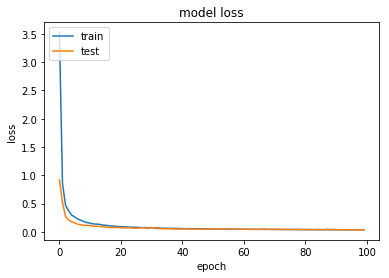
\includegraphics[scale=0.7]{figures/loss.png}
	\caption{Traningsfehler (train) und Validierungsfehler (val) über 100 Epochen}
	\label{img:loss}
\end{figure}

Festzustellen ist, dass beide Fehlerwerte sich zunächst stark fallend $0.0$ annähren und zwischen den Epochen $20-25$ und $100$ gleichbleibend $0.0$ zu sein scheinen. Aufgrund der Start-Traningsfehler von etwa $3.5$ lassen sich sehr kleine Werte nicht grafisch beurteilen. Ein direkter Blick auf die Fehlerwerte zeigt, dass beide sich im Bereich \num{10e-2} weiter $0.0$ annähern, mit dem Besten Validierungsfehler von $0.0344$ in Epoche $197$. Es besteht keine ausgeprägte Divergenz zwischen Trainings- und Validierungsfehler, das ist positiv zu beurteilen.\\
Bei kritischer Betrachtung muss angemerkt werden, dass die Regressionkurve, im konkreten Fall die Annäherung des Lenkwinkels, sehr rapide fällt. Dieses kann Zeichen eines Overfittings sein. Die Bilder der Teststrecke könnten in der Menge zu homogen sein, die Teststrecke ist im Angesicht der dort aufgenommenen Bildermenge relativ kurz, viele Bilder sind ähnlich mit nur leicht unterschiedlichen Lenkwerten. Aufgrund der räumlichen Abgeschlossenheit der Teststrecke gibt es dazu wenig Variabilität im Bildhintergrund, das könnte die Gleichartigkeit der Bilder verstärken.\\
Allerdings ist die schnelle Konvergenz nicht zwingend negativ anzumerken, das neuronale Netz war schließlich schon mit derselben Aufgabe auf einer ähnlichen Bildermenge trainiert worden. Dazu kommt, dass nur ein Teil der Layer überhaupt für das Traning, also eine Veränderung der Gewichte, freigegeben war. Im Angesicht dieser Umstände, können die Fehlerkurven in Abbildung~\ref{img:loss} auch für eine schnelle, effiziente Anpassung der Gewichte des letzten Residual-Blocks stehen.\\
Wie das CNN als Steuerungslogik in realen Szenarien abschneidet, wird in den nächsten Abschnitten untersucht.

\section{Testfahrt}
Um die Lenkwinkelbestimmung des Netzes zu Testen, wird zunächst frei auf der Strecke gefahren. Das Fahrzeug startet auf einer Geraden und fährt den Kurs überwiegend Fehlerfrei ab. Der Onboard-Rechner (NUC) des Fahrzeugs verarbeitet die Bilder mit $20 fps$, getestet wird bis zu einer Geschwindigkeit von \SI{1.2}{\meter/\second}, ab da nimmt die Lenkfehlerhäufigkeit stark zu. Ein Lenkwinkelupdate (verarbeiteter Frame) pro gefahrene $6 cm$ ist zum sauberen Fahren die Grenze.\\
\paragraph{Autonomiemetrik}
Die Fahrleistung auf der Strecke soll gemessen werden, um Sie direkt mit anderen Algorithmen vergleichen zu können. Dazu wird eine Autonomie-Metrik bestimmt \cite{bojarski2016end}. Der Autonomiewert wird definiert als 
\begin{equation}
\label{mat:autonomie}
(1 -  \frac{\text{Anzahl Fehler}\cdot 2 s}{\text{Fahrzeit in Sekunden}})\cdot 100,
\end{equation}
wobei die Anzahl der Fehler die Summe der Situationen ist, in der das Fahrzeug die Außen- oder Mittellinie mit mehr als zwei Reifen überquert hat. Das Fahrzeug kann sich danach selbst wieder auf die Strecke bringen, oder per Hand zurückgelenkt werden. Die Zeit, die vergeht, bis das Fahrzeug wieder sauber auf die Straße zurückgekehrt ist, wird mit 2 Sekunden angenommen. Die Fahrzeit in Sekunden beschreibt die Dauer des Versuchs.\\
Für den Test werden zwei Runden auf der Teststrecke gefahren, einmal im Uhrzeigersinn und einmal gegen den Uhrzeigersinn, beide Runden auf der jeweils Rechten Straßenseite. Als Geschwindigkeit wird \SI{1/2}{\meter/\second} festgelegt. In jede Richtung der Strecke wird $60$ Sekunden gefahren, das entspricht je einer Runde. Die Gesamtfahrzeit für alle Tests ist damit $120$ Sekunden.\\
Verglichen wird das unveränderte DroNet, die abgestimmte (finegetunte) Variante (bezeichnet als BA-RR) und der Steuerungsalgorithmus (Linienerkennung), der von der diesjährigen Carolo-Cup-Projektgruppe entwickelt wurde. Die erste Runde ist mit, die zweite gegen den Uhrzeigersinn. Die Testfahrten ergaben die in Tabelle~\ref{tab:testfahrten} gesammelten Daten.



\begin{table}[h]
  \begin{center}
    \caption{Algorithmen im Vergleich}
    \label{tab:testfahrten}
    \begin{tabular}{l|c|r} % <-- Alignments: 1st column left, 2nd middle and 3rd right, with vertical lines in between
      \textbf{Algorithmus} & \textbf{Fehler Runde 1} & \textbf{Fehler Runde 2}\\
      \hline
      DroNet & 16 & 12\\
      Carolo-Projekt & 7 & 11\\
       BA-RR& 3 & 5\\
    \end{tabular}
  \end{center}
\end{table}

Der Autonomiewert wird nach der Formel berechnet und liefert die in Tabelle~\ref{tab:autonomie} vermerkten Werte. Der Autonomiewert ist eine Prozentangabe und ist auf ganze Zahlen gerundet.

\begin{table}[h]
  \begin{center}
    \caption{Vergleich der Autonomie}
    \label{tab:autonomie}
    \begin{tabular}{l|r} % <-- Alignments: 1st column left, 2nd middle and 3rd right, with vertical lines in between
      \textbf{Algorithmus} & \textbf{Autonomiewert} \\
      \hline
      DroNet & 53 \% \\
      Carolo-Projekt & 70 \%  \\
       BA-RR& 87 \% \\
    \end{tabular}
  \end{center}
\end{table}

Der ursprüngliche DroNet Algorithmus ist nur $53 \%$ der Fahrzeit autonom unterwegs, was nicht überrascht, da er in einem anderen Anwendungsszenario entstand. Der Algorithmus des aktuellen Carolo-Projektteams ist deutlich besser, hat allerdings auch viele Fahrfehler gemacht. Die in dieser Arbeit entwickelte Steuerung (BA-RR) ist $87 \%$ der Fahrzeit autonom unterwegs, hier zeigt sich die deutliche Verbesserung, die insbesondere im Gegensatz zum DroNet Algorithmus erreicht wurde. Außerdem wird deutlich, das eine Steuerung mittels statistischer Auswertung von Bilddaten (CNN) nicht nur möglich ist, sondern einer Steuerung mittels klassicher Linienerkennung sogar überlegen sein kann. \\
Im Folgenden wird das Verhalten des Fahrzeugs in bestimmten Szenarien untersucht.

\section{Einzelszenarien}

\paragraph{Fahrbahn wiederfinden}
Im Hinblick auf die Eingangs angesprochene mögliche Overfitting-Problematik, wird hier eine praktische Herangehensweise an die Analyse gemacht.
Im Traningsbilderset sind keine Bilder enthalten, in denen das Fahrzeug aus einer Fehlersituation wieder auf die Straße navigiert. Genauer gesagt, in denen das Fahrzeug nicht oder nur teilweise auf der Strecke steht und den Weg in die richtige Fahrspur selbst findet. Somit konnten diese Szenarien beim Traning auch nicht \glqq auswendig \grqq{} gelernt werden. Diese Fehlersituationen werden jetzt künstlich erzeugt und das Fahrverhalten betrachtet.
Abbildung~\ref{fig:fehlerszenarien} zeigt Beispielhaft zwei solche Szenarien, einmal steht das Fahrzeug teilweise auf der Straße (\ref{fig:szena}), im anderen Beispiel steht es komplett außerhalb der Fahrbahn (\ref{fig:szenb}).


\begin{figure}[h]
	\centering
	\begin{subfigure}{.5\textwidth}
	\centering
		  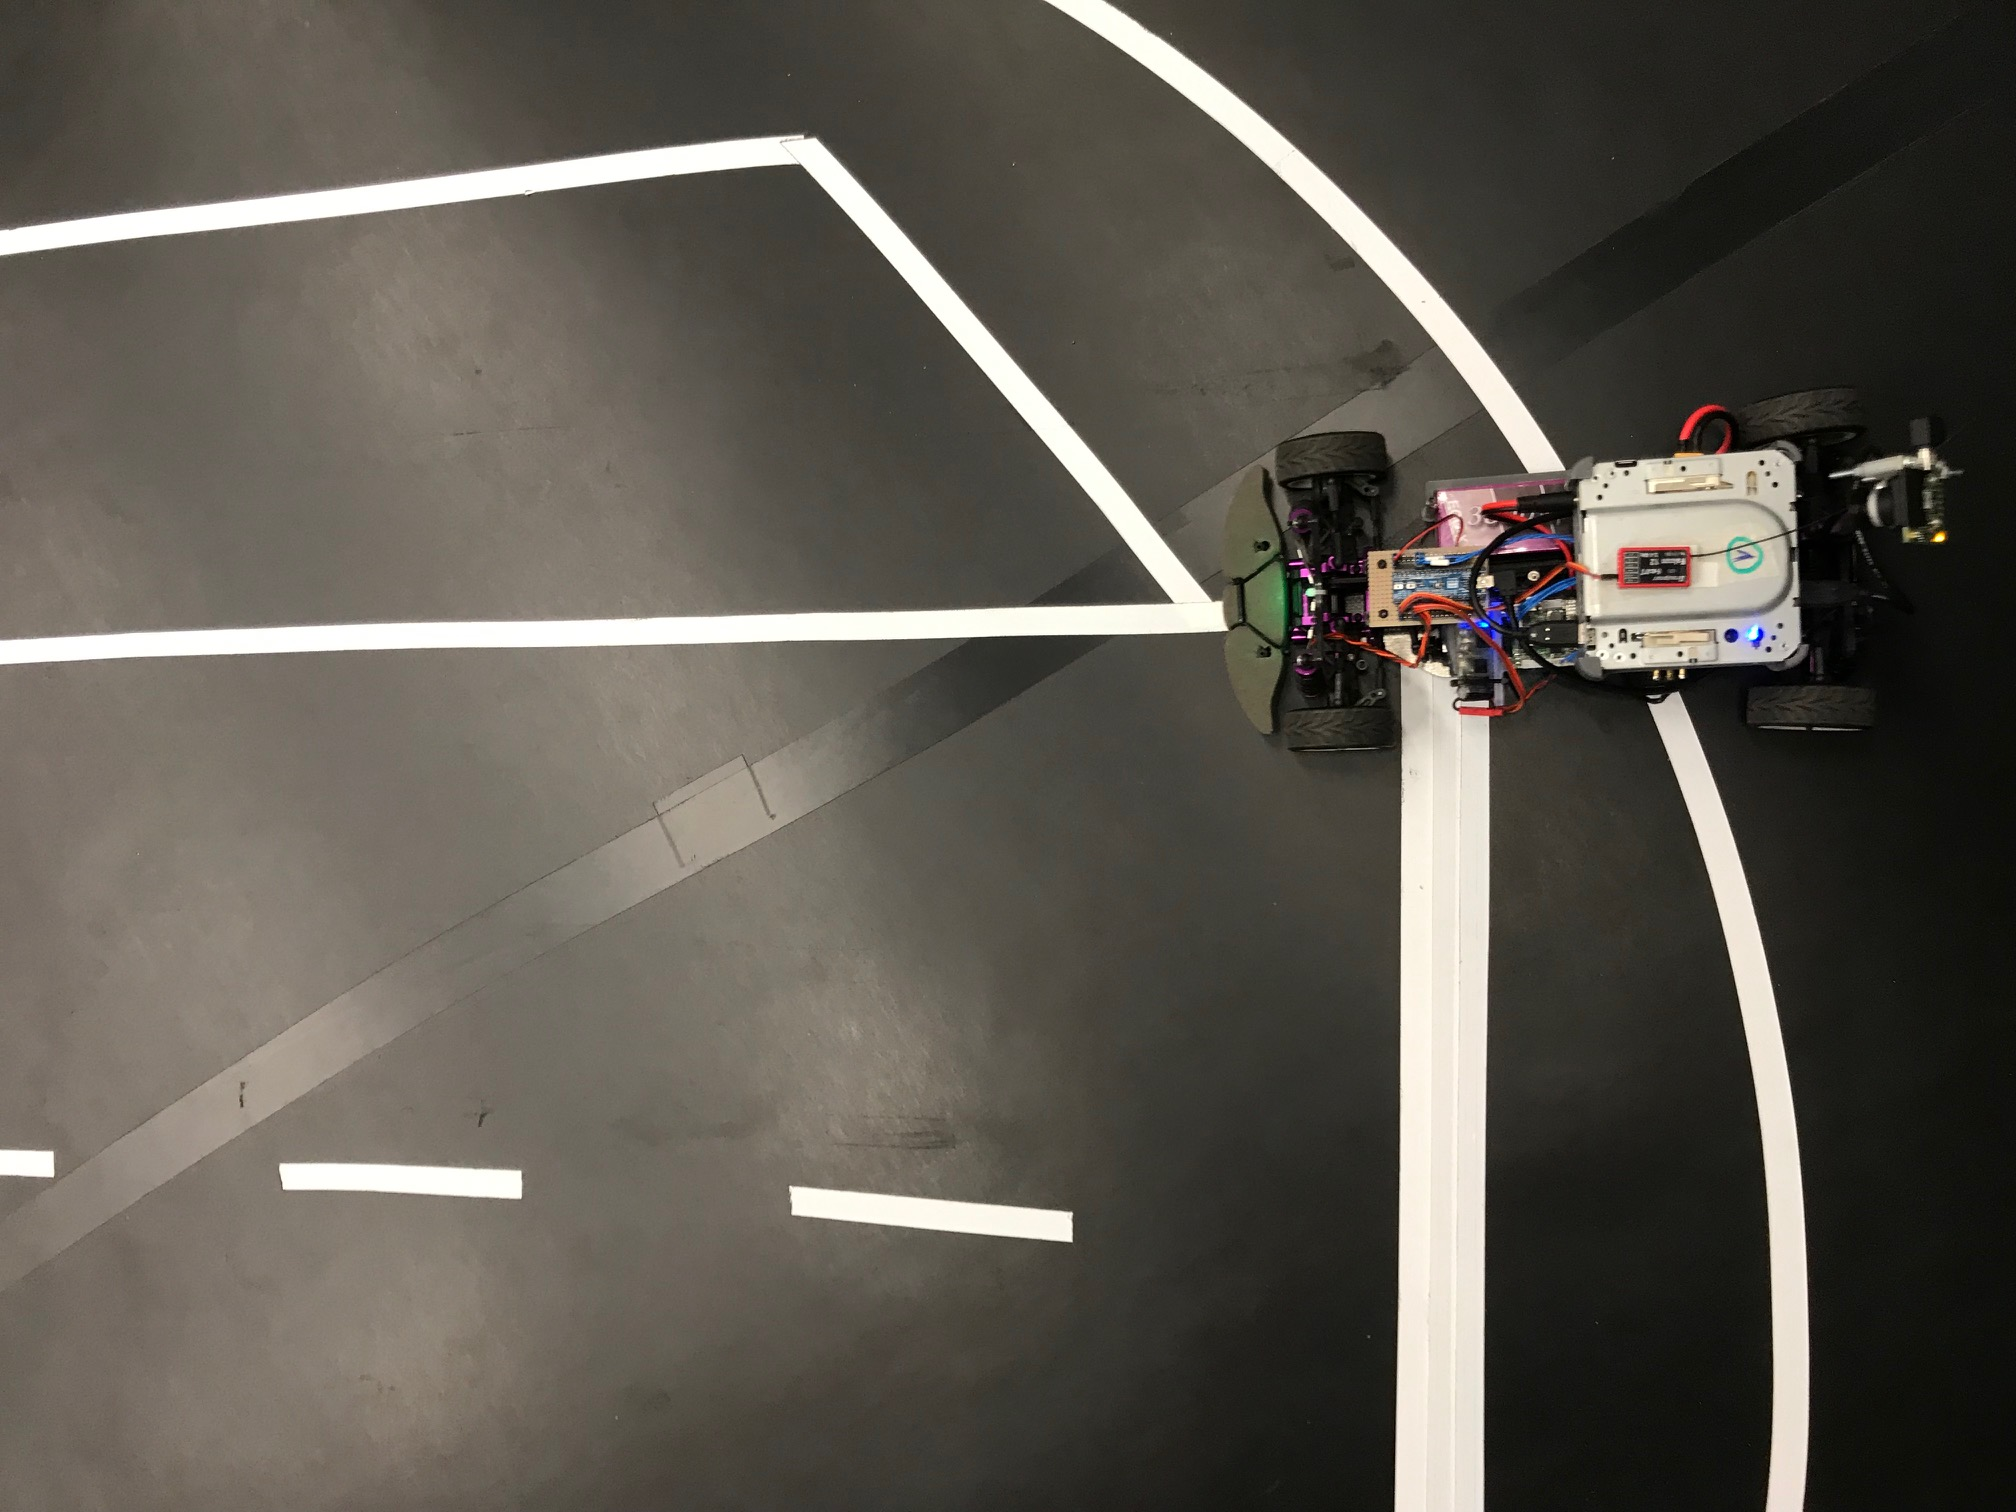
\includegraphics[width=0.8\linewidth]{figures/szenario1.jpg}
	 	  \caption{}
		  \label{fig:szena}
	\end{subfigure}%
	\begin{subfigure}{.5\textwidth}
	\centering
		  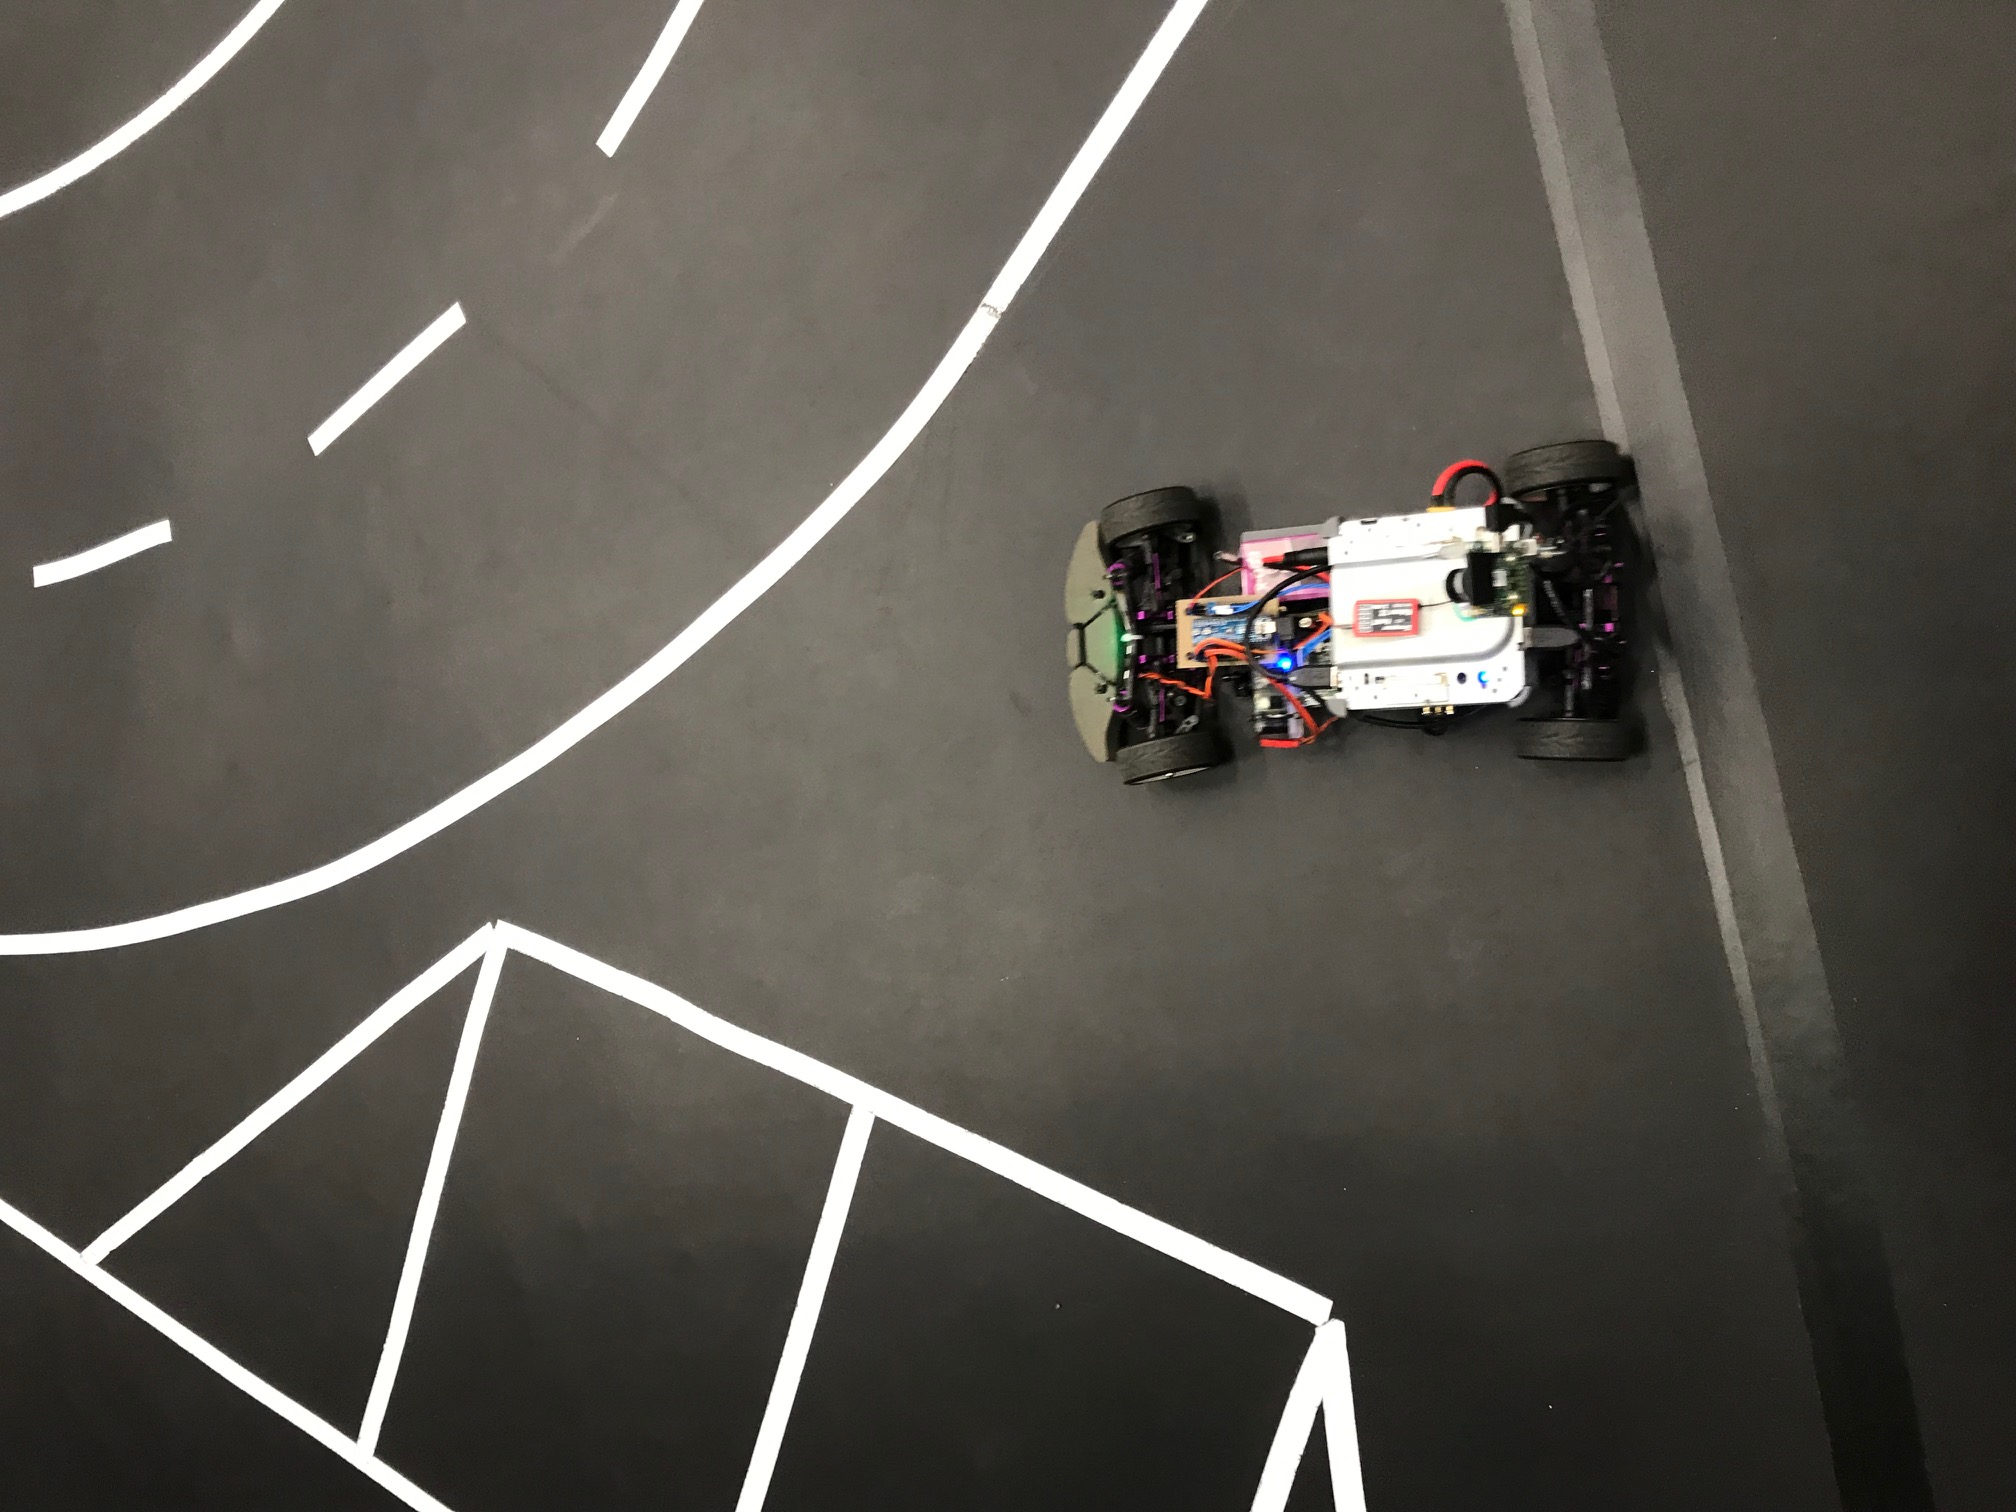
\includegraphics[width=0.8\linewidth]{figures/szenario2.jpg}
	 	  \caption{}
		  \label{fig:szenb}
	\end{subfigure}%
	\caption{Fehlerszenarien}
	\label{fig:fehlerszenarien}
\end{figure}%

Es wurden jeweils $10$ verschiedene Szenarien mit dem Fahrzeug teilweise auf der Fahrbahn und $10$ mit dem Fahrzeug außerhalb der Fahrbahn (jedoch mit Kamerasicht auf zumindest einen Teil der Fahrbahn) getestet. In $10/10$ Szenarien findet das Fahrzeug den Weg auf die Fahrspur, wenn es teilweise darauf steht. In $9/10$ Fällen findet es die Fahrspur, wenn es vollständig außerhalb der Fahrbahn steht.\\
Aus diesem Versuch lässt sich die Vermutung ableiten, dass die Orientierung an Fahrbahneigenschaften nicht nur in den trainierten Fällen funktioniert. Die Fahrspur wird auch aus vorher nicht gesehenen Blickwinkeln gefunden.

\paragraph{Kreuzung}
Da die Teststrecke nur eine Kreuzung hat, sind in den Traningsdaten sind nur wenige Bilder von Kreuzungsszenarien, wie dem in Abbildung~\ref{img:szenariokreuzung} gezeigten, vorhanden. Das Verhalten in diesen speziellen Situationen, in denen ein Teil der Fahrbahnmarkierung fehlt, ist besonders interessant.

\begin{figure}[h]
	\centering
	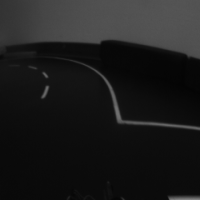
\includegraphics[scale=0.7]{figures/szenarioKreuzung.png}
	\caption{Kreuzungsszenario aus Sicht der Fahrzeugkamera}
	\label{img:szenariokreuzung}
\end{figure}

Tatsächlich erweisen sich die Kreuzungssituationen als größte Fehlerquelle. Wird die Kreuzung gerade angefahren, wird sie in $9/10$ Versuchen sauber überquert. Ist das Fahrzeug allerdings nicht mittig auf der Fahrbahn, sondern fährt die Kreuzung in einem leicht veränderten Winkel an, wird sie nur noch in $5/10$ Versuchen sauber durchfahren. In $50 \%$ der Testfälle mit leicht verändertem Blickwinkel verlässt das Fahrzeug die Fahrspur und wechselt die Spur.\\
Fehlt die Seitenlinie zur Orientierung, erschwert das die Lenkwinkelbestimmung. Durch eine leicht schräge Anfahrt der Kreuzung (zum Beispiel nach einer nicht ganz sauber durchfahrenen Kurve) gerät schnell die andere Fahrbahn in den Blickwinkel, welche dann zur Orientierung verwendet wird. Das Fahrzeug wechselt die Fahrspur.


\section{Saliency}
Gerade vor dem Hintergrund der Analyse des Netzes  ist es interessant zu Wissen, welche Bereiche des Bildes für die Bestimmung des Lenkwinkels tatsächlich von Bedeutung sind. Als Mensch kennt man das Konzept einer Fahrbahnmarkierung und der daraus entstehenden Fahrspur sehr genau. Man könnte davon ausgehen, dass für ein neuronales Netz diese Bereiche eines Bildes deswegen ebenfalls besonders interessant sind, um die Fahrtrichtung zu bestimmen.\\
Auch in Bezug auf die in vorangegangenem Kapitel besprochenen Problematiken, liegt ein gesteigertes Interesse vor, die wichtigen Bereiche der Fahrbahnbilder ausfindig zu machen.\\
Für die Visualisierung werden so genannte Saliency-Maps verwendet. Diese wurden 2013 in einem Papert \cite{simonyan2013deep} erstmals vorgestellt. Die Idee ist, jene Bildpunkte zu identifizieren, welche für die größten Veränderungen im Output sorgen. Für diese Arbeit bedeutet das, genau die Bildpunkte visuell hervorzuheben, welche für eine große Veränderung im Lenkwinkeloutput sorgen. Dafür wird die Veränderung (Gradient) des Outputs (Lenkwinkel) in Bezug auf das Eingabebild berechnet, also das Verhältnis einer Änderung im Output zu einer Änderung im Input: $\frac{\partial Output}{\partial Input}$.    Für diese Analyse wird Keras-vis \citeI{raghakotkerasvis} genutzt, eine Visualisierungs-API für Keras.\\
Um die Repräsentation der Bildeigenschaften im Netz deutlich zu machen, wird eine Saliency Map für jeden der drei Residual-Blöcke bestimmt. So lässt sich nachvollziehen, wie sich die ausschlaggebenden Bildbereiche auf dem Weg durch das Netz verändern. In Abbildung~\ref{img:saliency} sind diese drei Saliency Maps für ein Beispielbild einer Linkskurve dargestellt.\\
Die hellen Bildbereiche sind eben die, die für eine Erhöhung des Outputs sorgen, also für einen positiven Lenkwinkel. Zur Erinnerung, ein positiver Lenkwinkel codiert eine Linkskurve. Die Saliency-Map wurde für die jeweils letzte Convolutional-Layer des Blocks berechnet.

\begin{figure}[h]
	\centering
	\begin{subfigure}{\textwidth}
	\centering
		  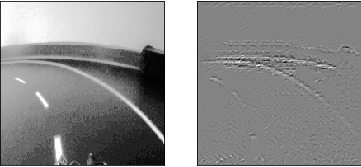
\includegraphics[width=0.8\linewidth]{figures/firstBlock.png}
	 	  \caption{Residual-Block 1}
		  \label{fig:saliena}
	\end{subfigure}\\
	\begin{subfigure}{\textwidth}
	\centering
		  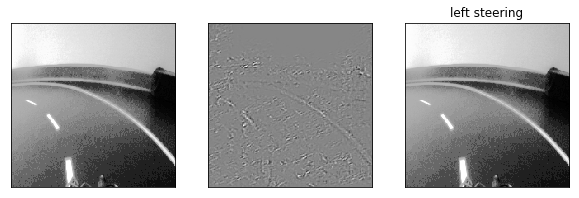
\includegraphics[width=0.8\linewidth]{figures/secondBlock.png}
	 	  \caption{Residual Block 2}
		  \label{fig:salienb}
	\end{subfigure}\\
	\begin{subfigure}{\textwidth}
	\centering
		  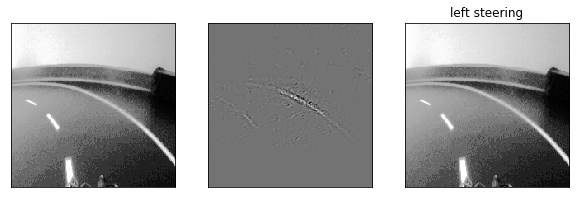
\includegraphics[width=0.8\linewidth]{figures/thirdBlock.png}
	 	  \caption{Residual Block 3}
		  \label{fig:salienc}
	\end{subfigure}%
	\caption{Ausschlaggebende Bildbereiche}
	\label{img:saliency}
\end{figure}%






